\documentclass[useAMS,usenatbib]{mn2e}

\voffset=-0.8in

% Packages:
\usepackage{graphicx}
\usepackage{amsmath}
\usepackage{xspace}
\usepackage{dsfont}

% Bold symbols
\renewcommand{\btheta}{\boldsymbol{\theta}}
\newcommand{\bdata}{\boldsymbol{D}}
\newcommand{\bx}{\{x_i\}}

% \onecolumn
%%%%%%%%%%%%%%%%%%%%%%%%%%%%%%%%%%%%%%%%%%%%%%%%%%%%%%%%%%%%%%%%%%%%%%%%%%%%%%

\title[]
{Fast Bayesian Inference for Exoplanet Discovery in Radial Velocity Data}
    
\author[Brewer]{%
  Brendon~J.~Brewer$^{1}$\thanks{bj.brewer@auckland.ac.nz},
  Courtney P. Donovan$^{1}$
  \medskip\\
  $^1$Department of Statistics, The University of Auckland, Private Bag 92019, Auckland 1142, New Zealand}

%%%%%%%%%%%%%%%%%%%%%%%%%%%%%%%%%%%%%%%%%%%%%%%%%%%%%%%%%%%%%%%%%%%%%%%%%%%%%%

\begin{document}
             
\date{To be submitted to MNRAS Letters}
             
\maketitle

\label{firstpage}

%%%%%%%%%%%%%%%%%%%%%%%%%%%%%%%%%%%%%%%%%%%%%%%%%%%%%%%%%%%%%%%%%%%%%%%%%%%%%%

\begin{abstract}
Inferring the number of planets $N$ in an exoplanetary system from radial velocity
(RV) data is a challenging task. Typically, the posterior distribution for the
planet parameters is multimodal and may have other awkward features. In
addition, when $N$ is unknown, the marginal likelihood (or evidence), as a
function of $N$, is required. In this paper we propose an alternative
approach using a trans-dimensional Markov Chain Monte Carlo method within
Nested Sampling. The posterior distribution for $N$ can be obtained with a
single run, which takes $\sim$ 15 minutes on a typical modern desktop computer.
We apply the method to $\nu$ Oph and Gliese 581, finding moderate evidence
(posterior probability of existence = 70\%) for a third planet around
$\nu$ Oph with an orbital period of 75.7 $\pm$ 1.8 days. 
\end{abstract}

\begin{keywords}
methods: data analysis
\end{keywords}

%%%%%%%%%%%%%%%%%%%%%%%%%%%%%%%%%%%%%%%%%%%%%%%%%%%%%%%%%%%%%%%%%%%%%%%%%%%%%%

\section{Introduction}
The number of known extrasolar planets has exploded in the last two
decades \citep{}. These discoveries have been driven by improvements in
all of the different techniques used to detect and characterise exoplanets,
including the radial velocity method \citep[e.g.][]{},
the transit method \citep[e.g.]{},
and gravitational microlensing
\citep[e.g.][]{2014ApJ...785..155B, 2014ApJ...790...14Y}. This paper focuses on the
radial velocity method.

Many authors have considered the problem of inferring the properties of an
exoplanetary system from observational data. With radial velocity data,
the expected signal due to an exoplanet is periodic, and the goal is to
infer the number of planets in the system, as well as their properties such
as orbital periods and eccentricities. Many
different techniques have been proposed. These techniques fall into two main
classes: i) those based on periodograms \citep[e.g.][]{},
and ii) those based on model fitting in the Bayesian inference framework,
to describe the uncertainties probabilistically.

\section{Inference}
Bayesian inference is the use of probability theory to describe uncertainty
\citep{}. In this framework, we approach data analysis problems by first
constructing a {\it hypothesis space}, which is the set of possible answers
to the problem we are considering. Normally, this is the set of possible
values of a vector of parameters $\btheta$ whose values we want
to know. We then assign probability distributions
called the {\it prior} and the {\it sampling distribution}. The prior
distribution $p(\btheta)$ describes
our initial uncertainty about which values of the parameters
$\btheta$ are plausible, and the
sampling distribution $p(\bdata | \btheta)$ describes
our initial uncertainty about the data set we're going to observe, as a
function of the unknown parameters $\btheta$.
When the data is known, our state of knowledge about the parameter is
updated from the prior $p(\theta)$ to the posterior distribution given by
Bayes' rule:
\begin{eqnarray}
p(\btheta | \bdata) &=&
\frac{p(\btheta)p(\bdata | \btheta)}
{p(\bdata)}
\end{eqnarray}
where the denominator, often called the {\it evidence} or
{\it marginal likelihood}, is given by:
\begin{eqnarray}
p(\bdata) = \int p(\btheta) p(\bdata | \btheta) d^N \btheta
\end{eqnarray}

The unknown parameters are:
\begin{eqnarray}
\left\{N, \boldsymbol{\alpha}, \{\boldsymbol{\phi}\}_{i=1}^N, y_0, s, \nu\right\}
\end{eqnarray}
where $\boldsymbol{\alpha} = \{\mu_T, \sigma_T, \mu_A\}$ are the
hyperparameters, and $\phi_i = \{\}$ are the properties of planet $i$.

The number of orbiting planets, $N$, is usually of significant interest.
Most authors have carried out the inference for $N$ by doing separate runs, one
for each possible value of $N$, and calculating the marginal likelihood
$p(\bdata | N)$ as a function of $N$
\citep[e.g.][]{2011MNRAS.415.2523G, 2014MNRAS.437.3540F, fengji}.

\begin{table*}
\begin{tabular}{|c|c|c|}
\hline
Quantity	&	Meaning		& Prior\\
\hline
$N$		& Number of planets	& Discrete Uniform$(0, 10)$\\
\hline
		&	Hyperparameters	&	\\
$\mu_T$		&			&	\\
\end{tabular}
\end{table*}

We used hierarchical priors because...

\section{Orbit Simulations}
The expected (noise-free) signal due to an exoplanet is periodic, but
non-sinusoidal when the orbit is not perfectly circular. The expected
shape of the variations can be obtained from mechanical considerations.
To save time, we pre-computed the properties of orbits as a function of
ellipticity.

Consider a test particle moving in the $x$-$y$ plane under the influence of a
point mass at the origin. The equations of motion for the particle are:
\begin{eqnarray}
\frac{d^2x}{dt^2} &=& -\frac{x}{r^3} \\
\frac{d^2y}{dt^2} &=& -\frac{y}{r^3} \\
\end{eqnarray}
where $r = \sqrt{x^2 + y^2}$. The ODEs can be solved for any given set of
initial conditions for $x$, $y$, $\frac{dx}{dt}$, and $\frac{dy}{dt}$ to yield
the shape of the orbit. To simulate orbits
of different ellipticities, we set the initial position to $(1, 0)$, and
the initial velocity to $(0, v)$ where $v \in [0.4, 1]$.
If $v=1$, the orbit is circular and as $v$ decreases the orbit becomes more
elliptical. For trial values of $v$ ranging from 0.4 to 1 in steps of 0.005,
we simulated an orbit using a leapfrog integrator, and saved the
velocities $\frac{dx}{dt}$ and $\frac{dy}{dt}$ as a function of time to disk.
These saved orbits were used as a lookup table for constructing the expected
signal $y(t)$ due to a single planet.
Because of the initial conditions used,
the simulated orbits were all horizontally
aligned.

\section{Reanalysis of $\nu$ Oph}
The $\nu$ Oph system is generally accepted to have two confirmed planets
\citep[e.g.][]{2011AIPC.1331..102Q, 2012PASJ...64..135S, fengji}, with periods
of $530.3$ and $3190$ days.

The posterior distribution for $N$, the number of planets, is shown in
Figure~\ref{fig:nu_oph_N}.

The posterior distribution for the logarithms of the periods is shown in
Figure~\ref{fig:nu_oph_periods}. Because of the label-switching degeneracy,
the posterior samples for all periods were combined to make this figure, which
shows three prominent peaks. Defining the log-periods by
$S_i =  \log_{10}(T/\textnormal{1 day})$,
Figure~\ref{fig:nu_oph_periods} is a Monte Carlo representation
of the mixture distribution
\begin{eqnarray}
f(S) &=& \sum_{N=1}^{10} \frac{1}{N}\sum_{i=1}^N p(S_i | N, \bdata).
\end{eqnarray}


\begin{figure}
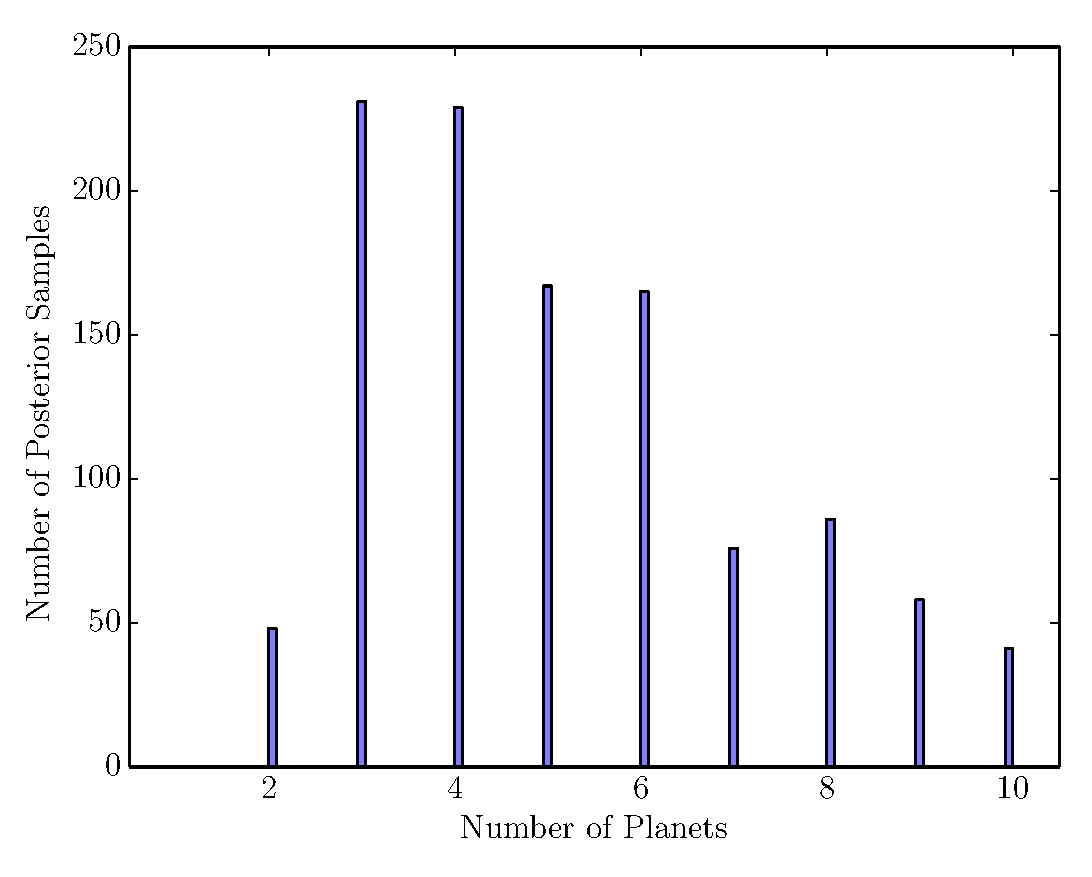
\includegraphics[scale=0.5]{Figures/nu_oph_N.eps}
\caption{The posterior distribution for the number of planets $N$ orbiting
$\nu$ Oph.\label{fig:nu_oph_N}}
\end{figure}

\begin{figure}
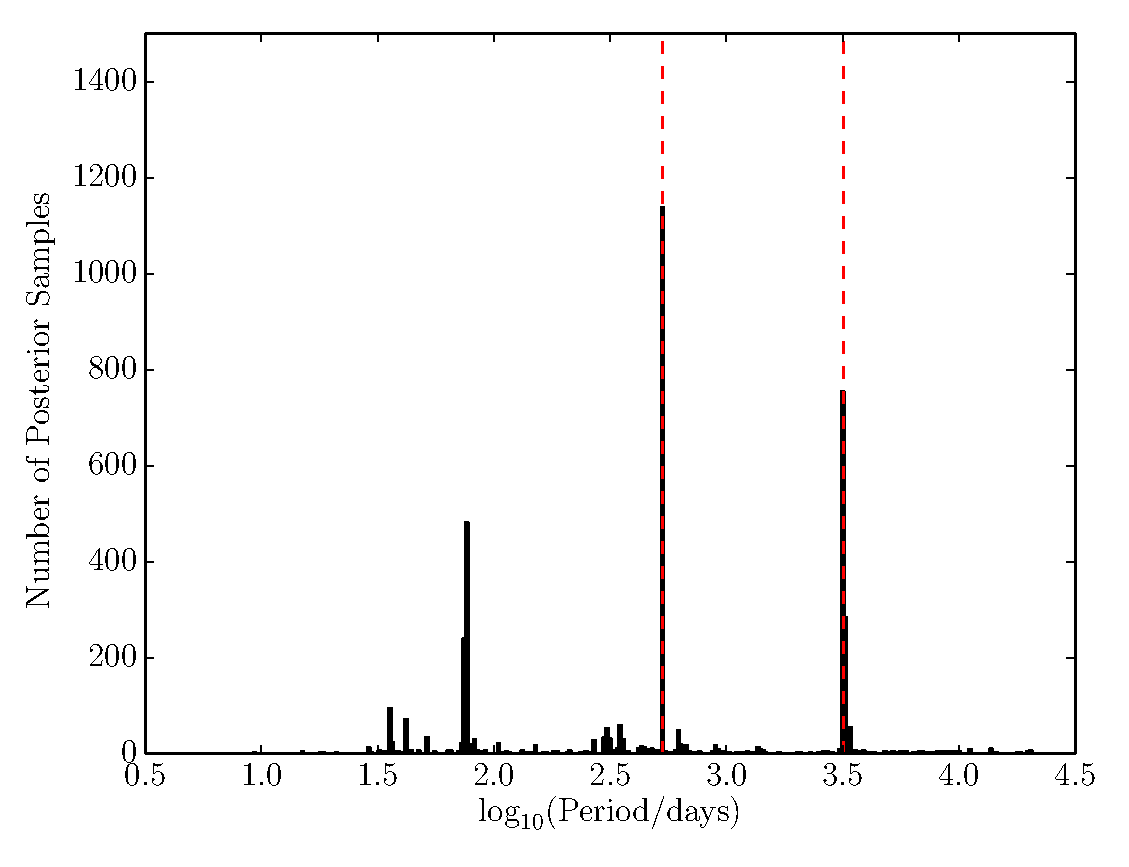
\includegraphics[scale=0.5]{Figures/nu_oph_periods.eps}
\caption{The posterior distribution for the orbital periods in the $\nu$ Oph
system.\label{fig:nu_oph_periods}}
\end{figure}

\begin{figure}
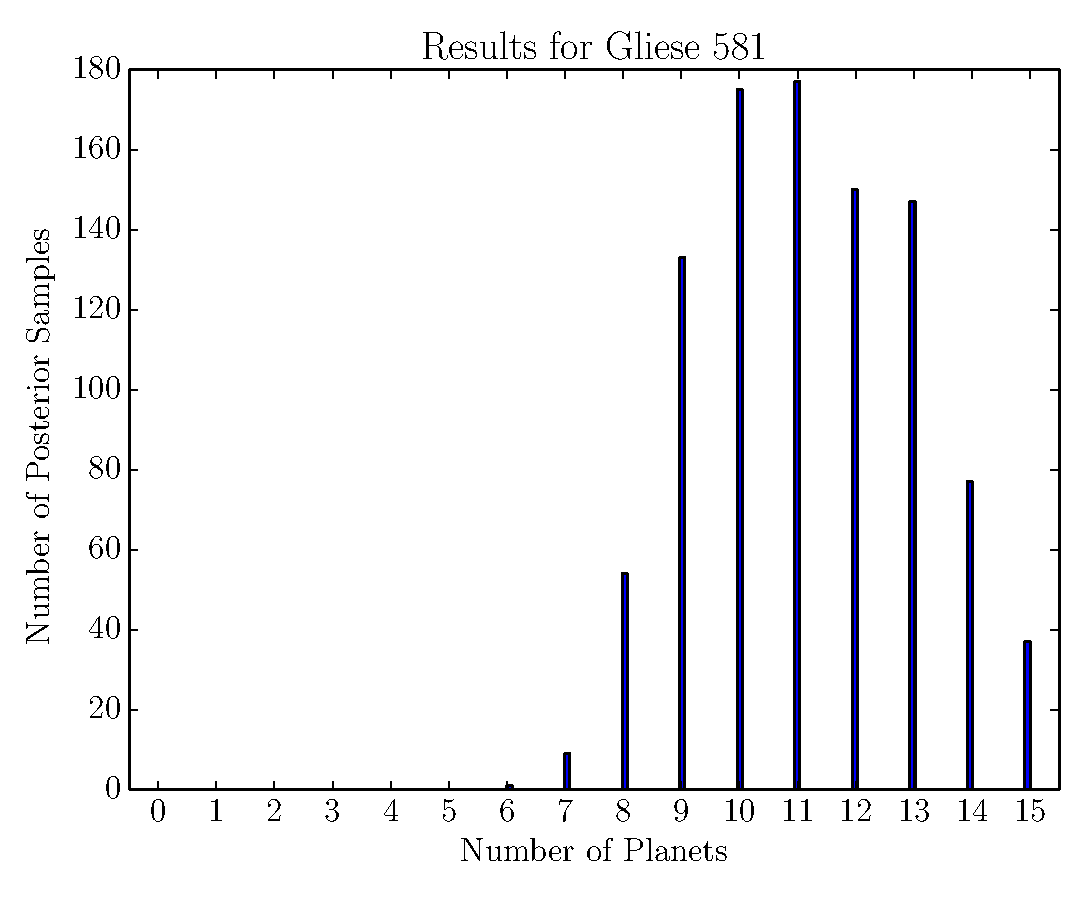
\includegraphics[scale=0.5]{Figures/gliese581_N.eps}
\caption{The posterior distribution for the number of planets $N$ orbiting
Gliese 581.\label{fig:gliese581_N}}
\end{figure}

\begin{figure}
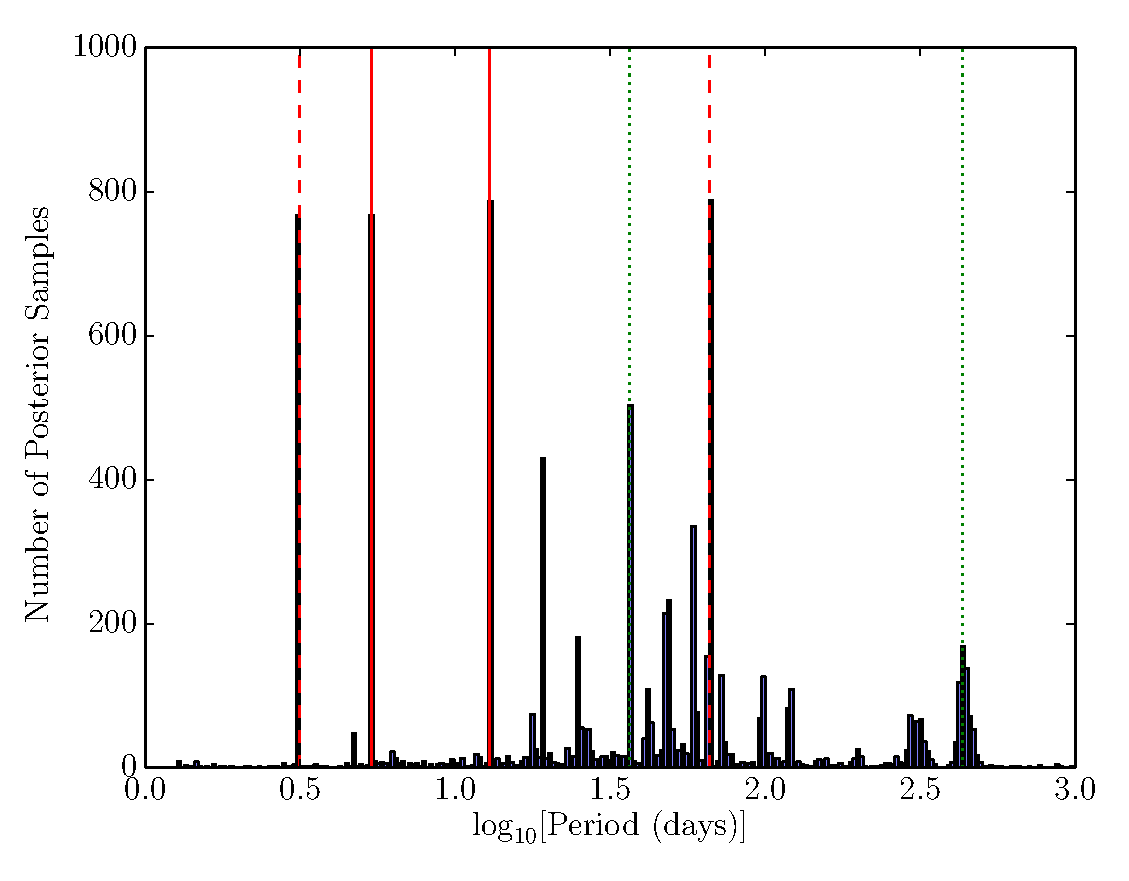
\includegraphics[scale=0.5]{Figures/gliese581_periods.eps}
\caption{The posterior distribution for the orbital periods in the Gliese 581
system.\label{fig:gliese581_periods}}
\end{figure}

\vspace{-0.5cm}
\section*{Acknowledgements}
It is a pleasure to thank Fengji Hou and David Hogg (NYU) for inspiring me to
finally work on this problem, and Phil Gregory (UBC) for writing so many
interesting papers on it. This work was supported by a Marsden Fast Start
grant from the Royal Society of
New Zealand.

\begin{thebibliography}{99}

\bibitem[\protect\citeauthoryear{Bennett et 
al.}{2014}]{2014ApJ...785..155B} Bennett D.~P., et al., 2014, ApJ, 785, 155 

\bibitem[\protect\citeauthoryear{Feroz 
\& Hobson}{2014}]{2014MNRAS.437.3540F} Feroz F., Hobson M.~P., 2014, MNRAS, 437, 3540 

\bibitem[\protect\citeauthoryear{Gregory}{2011}]{2011MNRAS.415.2523G} 
Gregory P.~C., 2011, MNRAS, 415, 2523 

\bibitem[\protect\citeauthoryear{Hou, Goodman, 
\& Hogg}{2014}]{fengji} Hou F., Goodman J., Hogg D.~W., 2014, arXiv, arXiv:1401.6128 

\bibitem[\protect\citeauthoryear{Quirrenbach, Reffert, 
\& Bergmann}{2011}]{2011AIPC.1331..102Q} Quirrenbach A., Reffert S., Bergmann C., 2011, AIPC, 1331, 102 

\bibitem[\protect\citeauthoryear{Sato et al.}{2012}]{2012PASJ...64..135S} 
Sato B., et al., 2012, PASJ, 64, 135 

\bibitem[\protect\citeauthoryear{Yee et al.}{2014}]{2014ApJ...790...14Y} 
Yee J.~C., et al., 2014, ApJ, 790, 14 

\end{thebibliography}



\end{document}

%%%%%%%%%%%%%%%%%%%%%%%%%%%%%%%%%%%%%%%%%%%%%%%%%%%%%%%%%%%%%%%%%%%%%%%%%%%%%%
